%        File: ubiquitous-location-based-service_cn.tex
%     Created: Sun Jan 01 03:00 PM 2012 C
% Last Change: Sun Jan 01 03:00 PM 2012 C
%
\documentclass{article}
\usepackage{CJKutf8}

% Package & settings for graphic
\usepackage[pdftex]{graphicx}
\usepackage{subfig} % Enable sub figure
\graphicspath{./figure/}
\DeclareGraphicsExtensions{.png,.jpg,.jpeg,.pdf}

% Package for References & Cite
\usepackage{natbib}
% Package for figures that not float
\usepackage{caption}

\title{无处不在的基于位置服务}
\author{Jae-Chul Kim, Tae-Wook Heo, Ju-Wan Kim, and Jong-Hyun Park}


\begin{document}
\begin{CJK}{UTF8}{gbsn}
	% Make title
  \maketitle

	% Rename
  \renewcommand{\abstractname}{摘要}
	\renewcommand{\figurename}{图}
	\renewcommand{\refname}{参考文献}

	% References style & cite settings
	\bibliographystyle{unsrtnat}
	\setcitestyle{super, square, aysep={}, yysep={;}}

	% Begin content
  \begin{abstract}
	鉴于Web服务环境提供了准确获取请求信息的方法,本论文中,我们提出了基于Web服务开发的无处不在的基于位置服务(Location Based Service, 简称:LBS)。该服务架构能够与开放位置服务标准(Open Location Service,简称:OpenLS)(目录服务、位置工具服务和路径服务)、追踪服务和旅游咨询服务配合使用。就此,我们提出了无处不在的基于位置服务的新架构解决方案。
  \end{abstract}

  \newpage
  \section{引言}
	通常,为了能够使用为不同业务流程设计的组件,往往会在已有的模块基础上进一步构建成大型应用。而使用面向服务的方法不仅能够规范交互性,而且在事务处理过程中提供了更大的灵活性。因此,一个面向服务的架构必须把重心放在如何描述和组织服务上,以支持动态性、自动查找和使用性。如果服务变得越来越复杂,那么基本的“请求-响应”机制就会变得难以运用了。一些中期甚至长期的服务需要一个合适的功能,以实现分别为用户和响应的服务(或者两个服务)之间建立一个异步通信\cite{LimWen}。而Web的消息通知服务正满足以上这些需求。Web服务是自包含的、模块化的服务应用,它可以通过网络描述、发布、定位,以及调用。从简单的“请求-响应”处理到完整的业务流程的交互,Web服务均采用封装的事务功能\cite{ScottBenRomin}。

	我们提出的服务架构所采用的新型LBS基础核心服务是基于Web服务构建的,从而克服了平台依赖性、系统封闭性,以及分布式计算环境等带来的限制。


	\section{Web服务系统}
	目前,W3C提出的Web服务标准如下:采用XML(eXtensible Markup Language,超文本标记语言)作为几乎所有Web服务规范基础的标记语言。XML是一种Web开发的常用语言,它可以将自身携带的任何数据内容解析到特定的设备,并以结构化方式显示数据信息\cite{DavidKurtChris}。SOAP(Simple Object Access Protocol,简单对象存取协议)是一个网络、传输和程序语言之间的协议,它允许客户端发送XML格式的消息\cite{TR1}来调用远程服务。WSDL(Web Services Description Language,网络服务描述语言)\cite{TR2}是一种基于XML接口和实现的描述语言。为了指定Web服务提供的操作,包括进行这些操作所需的参数和数据类型,服务提供商常选择使用WSDL文档(技术报告:Web Services Description Language 1.1)来规范。另外,一份WSDL文档通常还包含服务访问信息(技术报告:Web Services Description Language)。UDDI(Universal Description, Discovery, and Integration,统一描述、发现和集成)是一个客户端API,同时也是一个基于SOAP的服务器的实现,它可以存储和检索服务提供商和Web服务的信息。
	\begin{figure}[htbp]
		\centering
		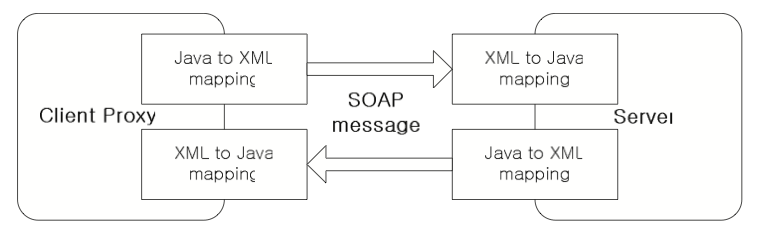
\includegraphics[bb=0 0 760 234, scale=0.45]{figure/fig01.png}
		\caption{Web服务的基本架构}
	\end{figure}

	同时,Java的XML包为运行Web服务提供了许多扩展API:JAXP(Java API for XML Processing,Java中处理XML的API)是一个面向文档的API,通过一个“可插拔(pluggability)”层,它允许在应用程序中使用任何兼容XML的解析器。JAXM(Java API for XML Messaging,Java中为XML消息传递机制提供的API)为开发产生和使用SOAP的程序提供了便捷,它提供了如创建SOAP消息、添加内容到SOAP消息中等函数方法。JAXR(Java API for XML Registries,Java中为XML注册机制提供的API)为访问中不同类型的注册提供了统一的方式。目前,JAXR同时支持ebXML和UDDI的注册。JAXR不仅含有发布、搜索、修改和删除注册表中的项的功能,还自带一些可浏览的JAXR客户端例子,如微软和IBM访问注册示例。JAX-RPC(Java API for XML-Based RPC,Java中为基于XML的RPC提供的API)提供了构建基于RPC和XML的Web服务和客户端的API。虽然它使用SOAP消息,但实际上,应用程序并不处理SOAP的消息部分(比如采用JAXM的情况下)。
	\begin{figure}[htbp]
		\centering
		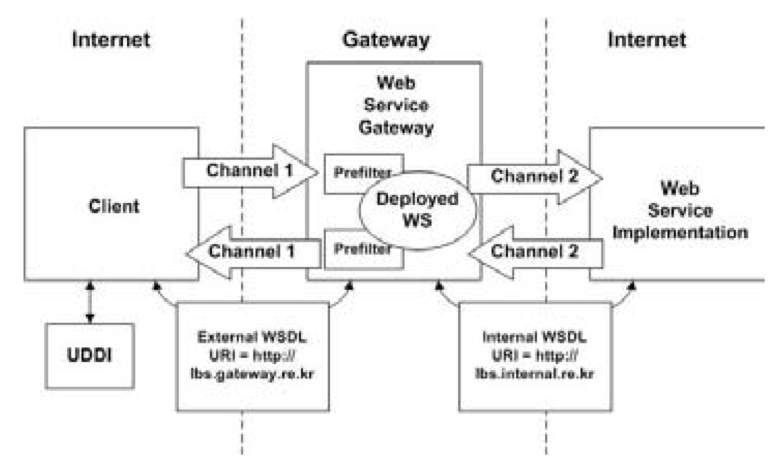
\includegraphics[bb=0 0 774 466, scale=0.45]{figure/fig02.png}
		\caption{Web服务的映射和解码}
	\end{figure}


	\section{系统架构}
	\subsection{OGC(Open GIS Consortium,开放地理信息联盟)顶层架构}
	\begin{figure}[htbp]
		\centering
		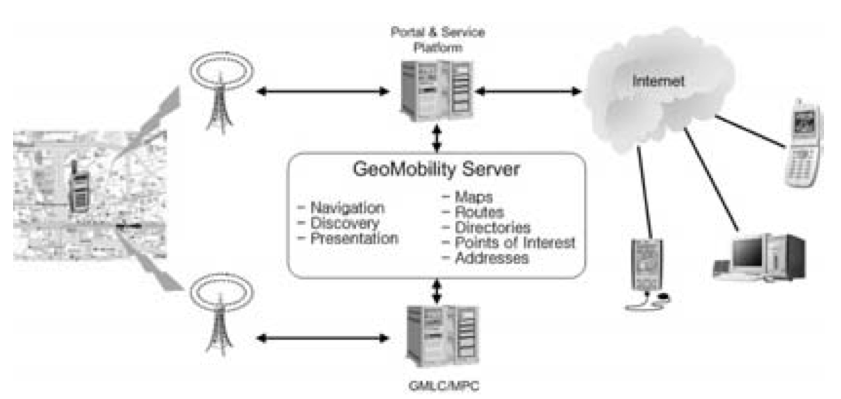
\includegraphics[bb=0 0 841 399, scale=0.45]{figure/fig03.png}
		\caption{为用户提供LBS应用服务(OGC)}
		\label{fig:OGC}
	\end{figure}

	为了满足在新兴的无线互联网市场中为用户提供挖掘丰富的空间内容,以及促进定位应用服务的发展这些需求,OGC提出并已形成开放位置服务(Open Location Services,简称OpenLS)的倡议。OpenLS的愿景是提供开方式的接口,以实现互操作性,并且让任何设备随时随地都可在周边的服务热点中提供可操作、多任务、分布式、增值的定位服务和内容成为可能。

	如图\ref{fig:OGC}所示为GeoMobility服务器和它所涉及的LBS架构中的其它元素组成的概念框架图。GeoMobility服务器是一个提供基本服务功能的服务器,LBS应用便托管在该服务器上(采用OpenLS核心服务)。该服务器采用开方式的接口实现访问网络位置的功能,并提供另外一些接口,使得托管在该服务器(或另一台服务器)上的应用能够访问OpenLS的核心服务。GeoMobility服务器除了能够提供诸如地图、路径、地址、感兴趣的点、交通等内容外,它还可以通过互联网访问本地的内容数据库。

	\subsection{开放式LBS基本核心组件架构}
	\begin{figure}[htbp]
		\centering
		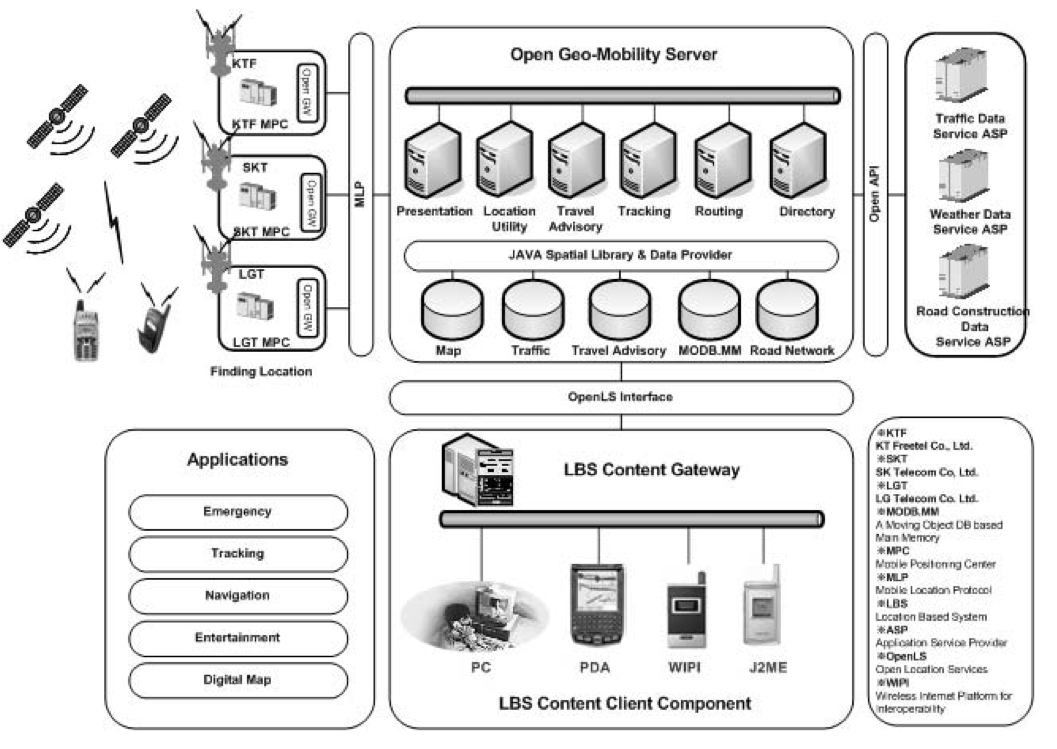
\includegraphics[bb=0 0 1057 749, scale=0.4]{figure/fig04.png}
		\caption{系统架构}
		\label{fig:system-architecture}
	\end{figure}

	如图\ref{fig:system-architecture}所示,LBS的基本核心组件与LBS平台相连,同时,核心服务的接口实现中包含Web服务。该系统包含Web服务器和由EJB(Enterprise Java Beans)开发的客户端两部分。开发工具为WSAD(Websphere Studio Application Developer)5.0,Web服务器采用WAS(Websphere Application Server)5.0。服务平台上考虑到互操作性的接口是基于OpenLS Spec.\cite{OpenLS, OpenLS2, OpenLS3} v.0.2版本实现的。每个CP(Content Provider,内容提供商)网关通过与LBS平台通信访问LBS基本核心组件,同时,通过采用JSP和Servlet与其客户端进行通信。

	图\ref{fig:system-architecture}展示了GeoMobility服务器和它相关的其它LBS架构元素之间是如何架构的。GeoMobility服务器是一个提供基本服务功能的服务器,LBS应用便托管在该服务器上(采用OpenLS核心服务)。该服务器采用开放式的接口实现访问网络位置的功能,并提供另外一些接口,使得托管在该服务器(或另一台服务器)上的应用能够访问OpenLS的核心服务。GeoMobility服务器除了能够提供诸如地图、路径、地址、感兴趣的点、交通等内容外,它还可以通过互联网访问本地的内容数据库。

	\subsection{开放式LBS基本核心组件}
	目录服务为用户提供了通过访问在线目录查找最近或特定的地方、产品、服务,通过使用含有OpenSL的应用,用户可以通过输入名称、类型、类别、关键字、电话号码,或其它“用户友好”(user-friendly)的标识符,来制定服务请求的搜索参数。当用户在一个特定的位置或区域搜索最近的(或期望的)地方、产品或服务时,发送的服务请求必须包含该用户的位置点信息。

	\begin{figure}[htbp]
		\centering
		\subfloat[请求] {
		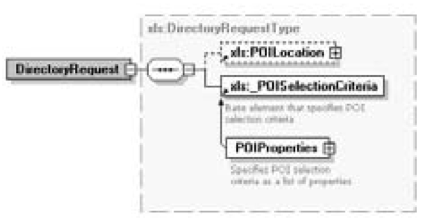
\includegraphics[bb=0 0 432 223, scale=0.35]{figure/fig05a.png}
		\label{fig:schema-of-directory-service-a}
		}
		\hspace{10pt} % Adjust sub figures margin space
		\subfloat[响应] {
		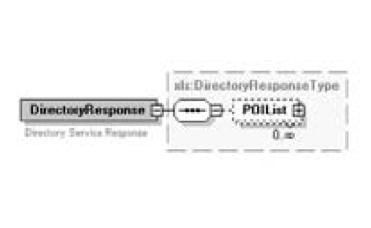
\includegraphics[bb=0 0 371 228, scale=0.35]{figure/fig05b.png}
		\label{fig:schema-of-directory-service-b}
		}
		\caption{目录服务架构}
	\end{figure}

	位置点可以是网关服务定义的移动终端的所在位置,也可以是以其它方式定义的一个远程位置。而目录也可以被特殊到某一具体内容(比如,黄页、餐厅指南等)。通过发送包含制定参数的请求,目录服务根据搜索条件搜索响应的联机目录,以响应对应的请求,比如寻找最近的(或特定的)的地方、产品或服务。最终,服务器响应并返回一个或多个查询结果列表(根据目录内容,提供位置信息,对该地方、产品或服务的详细描述信息等),不仅如此,该查询结果列表还将根据搜索条件进行有序地排列后显示给用户。
	
	\begin{figure}[htbp]
		\centering
		\subfloat[请求] {
		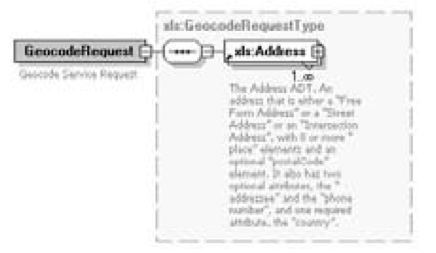
\includegraphics[bb=0 0 436 253, scale=0.35]{figure/fig06a.png}
		\label{fig:schema-of-location-utility-service-a}
		}
		\hspace{10pt}
		\subfloat[响应] {
		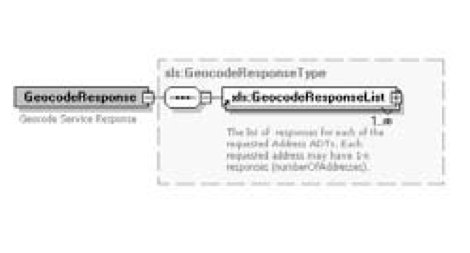
\includegraphics[bb=0 0 470 253, scale=0.35]{figure/fig06b.png}
		\label{fig:schema-of-location-utility-service-b}
		}
		\caption{位置实用工具服务架构}
	\end{figure}

	位置实用工具服务(Location-Utility Service)不仅可将地名、街道的地理位置、地址或邮政编码等转换成地理位置点(地理编码),还可以返回一个完整的、规范的地理描述(这在当只有部分信息已知的情况下是非常有用的)。该服务同时也提供将地理位置点反向转换成地名、街道地址、邮政编码等完整的、规范的地理描述(反向地理编码)。地理编码和反向地理编码操作都可能返回零个、一个或多个服务请求的响应,而这取决与用户的请求信息、采用的算法,以及内容的匹配程度。

	\begin{figure}[htbp]
		\centering
		\subfloat[请求] {
		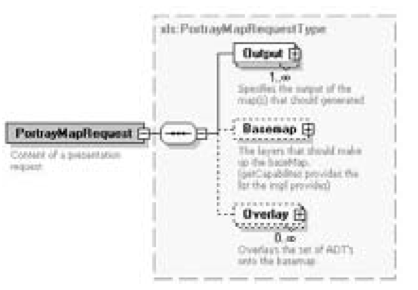
\includegraphics[bb=0 0 418 290, scale=0.35]{figure/fig07a.png}
		\label{fig:schema-of-presentation-service-a}
		}
		\hspace{10pt}
		\subfloat[响应] {
		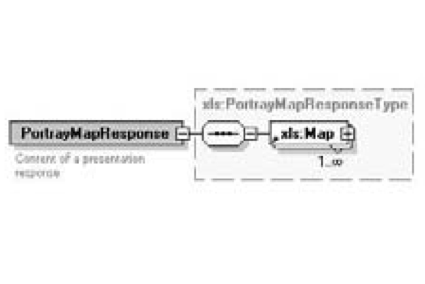
\includegraphics[bb=0 0 425 284, scale=0.35]{figure/fig07b.png}
		\label{fig:schema-of-presentation-service-b}
		}
		\caption{展示服务架构}
	\end{figure}

	展示服务将移动终端中的地理信息进行渲染处理后显示给用户。任何OpenLS应用程序都可以调用此服务以获得期望显示的区域地图,该地图还可以通过多个层的叠加描绘一个或多个OpenLS ADT(Abstract Data Types,抽象数据类型),比如:几何路线,感兴趣的位置点、区域,地址等。该服务也可用于呈现机动路线ADT列表或交通路线指示ADT列表的路线方向。

	\begin{figure}[htbp]
		\centering
		\subfloat[请求] {
		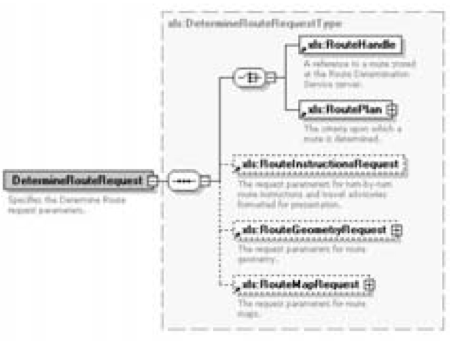
\includegraphics[bb=0 0 463 346, scale=0.35]{figure/fig08a.png}
		\label{fig:schema-of-route-service-a}
		}
		\hspace{10pt}
		\subfloat[响应] {
		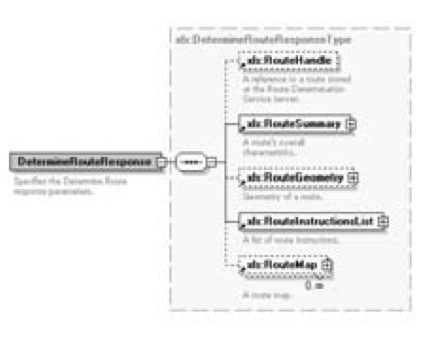
\includegraphics[bb=0 0 425 345, scale=0.35]{figure/fig08b.png}
		\label{fig:schema-of-route-service-b}
		}
		\caption{路径导航服务架构}
	\end{figure}

	路径导航服务为用户提供推荐的路径,用户必须使用导航类应用以使用该服务。用户必须指明起始位置(通常该位置通过网关服务获得,但这也可以是某条计划路线的特定起点位置,比如用户家门口)和终点位置(这可以是任何地方,比如只知道与该位置相关的电话号码或者地址的地方,又或者是通过目录服务搜索到的地方),除此之外,还可以选择特殊的路径点、路径的类别(最快的、最短的、交通堵塞程度最小的,或者沿途风景最美的,等等)和喜欢的交通方式。用户可以根据需要将路径存储到设备中,因此路径导航服务请求也会抓取存储的路径进行比较,从而提供更理想的路径。

	\begin{figure}[htbp]
		\centering
		\subfloat[请求] {
		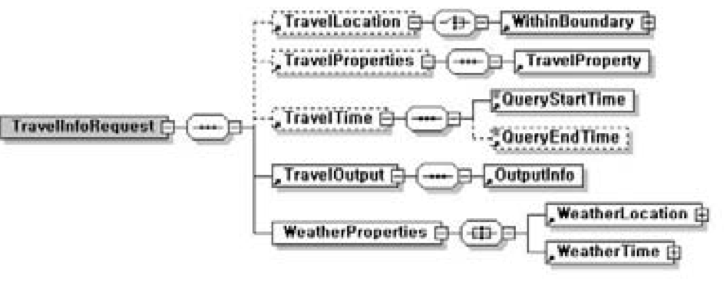
\includegraphics[bb=0 0 726 285, scale=0.35]{figure/fig09a.png}
		\label{fig:schema-of-travel-advisory-service-a}
		}
		\hspace{10pt}
		\subfloat[响应] {
		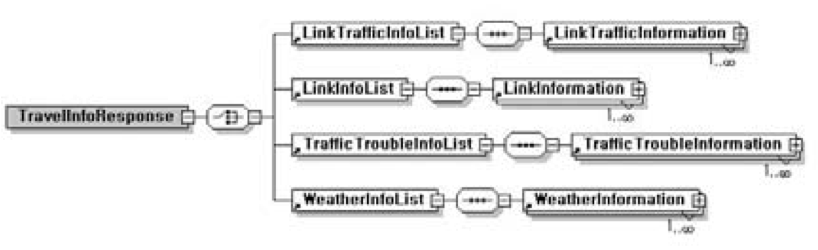
\includegraphics[bb=0 0 818 250, scale=0.35]{figure/fig09b.png}
		\label{fig:schema-of-travel-advisory-service-b}
		}
		\caption{旅游咨询服务架构}
	\end{figure}

	支持旅游咨询服务的个人导航应用可以通过使用该服务,对当前位置和目标位置的天气状况及将来的天气状况进行查询,该查询操作还可以获取道路和交通情况等数据。此外,个人导航应用还将跟踪用户的当前位置,通过将该服务和旅游咨询服务结合,根据旅游咨询服务提供的不断变化的交通和天气状况,近实时地向用户发出建议消息。

	在此,我们使用一个配备有GPS无线通讯功能的物理实体和一台计算机(比如PDA和移动电话)来跟踪物体的移动。

	\begin{figure}[htbp]
		\centering
		\subfloat[请求] {
		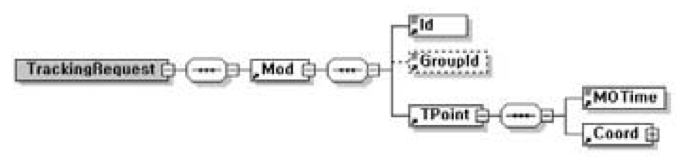
\includegraphics[bb=0 0 697 164, scale=0.35]{figure/fig10a.png}
		\label{fig:schema-of-traffic-service-a}
		}
		\hspace{10pt}
		\subfloat[响应] {
		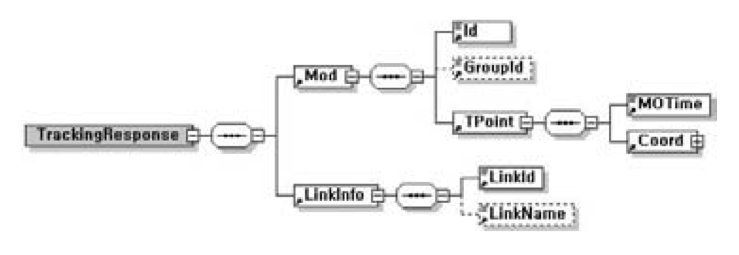
\includegraphics[bb=0 0 739 255, scale=0.35]{figure/fig10b.png}
		\label{fig:schema-of-traffic-service-b}
		}
		\caption{交通服务架构}
	\end{figure}

	我们观察到,该移动物体的实际轨迹是由系统产生的许多个点相互作用产生的,而不是单单一条线段。我们采用卡尔曼滤波算法\cite{BrownPYC}调整不确定的移动对象,在某一状态下运行一段时间后获得测量形式(噪音)的反馈。

	\begin{figure}[htbp]
		\centering
		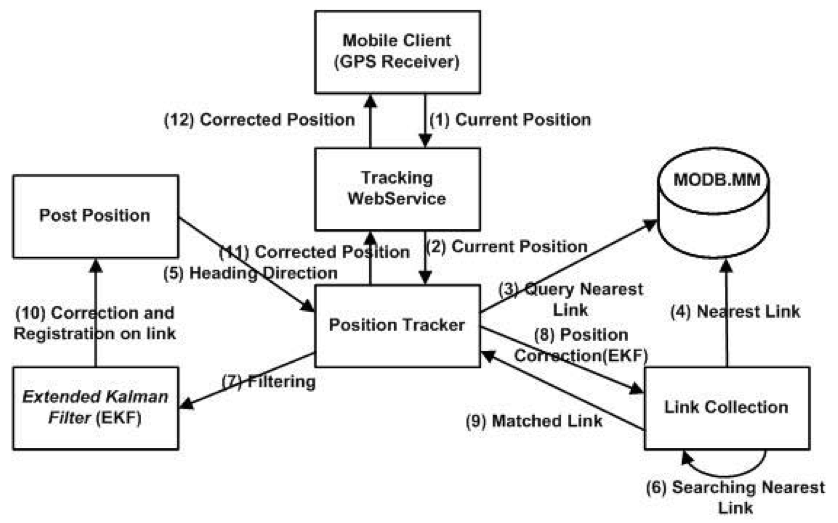
\includegraphics[bb=0 0 838 523, scale=0.45]{figure/fig11.png}
		\caption{位置矫正算法}
		\label{fig:position-correction-algorithm}
	\end{figure}


	\section{LBS基本核心组件的客户端}
	开发的客户端经过在有线和无线的环境下测试。客户端平台为PDA(Microsoft WindowsCE,iPAQ5550)和WIPI手机(WIPI,SamSung X9300,Arm9,4MB)。

	\noindent\begin{minipage}{\textwidth}
		\centering
		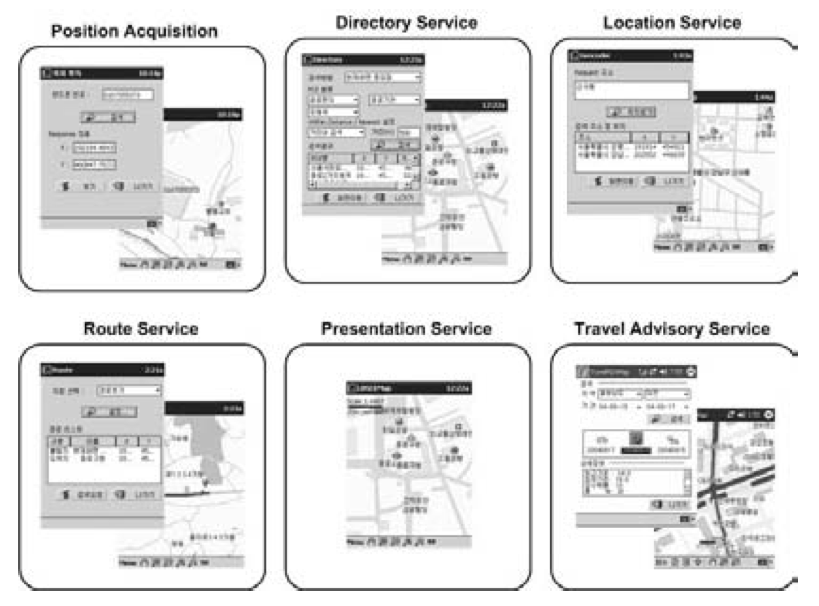
\includegraphics[bb=0 0 819 606, scale=0.45]{figure/fig12.png}
		\captionof{figure}{LBS PDA客户端(WinCE)}
	\end{minipage}

	\noindent\begin{minipage}{\textwidth}
		\centering
		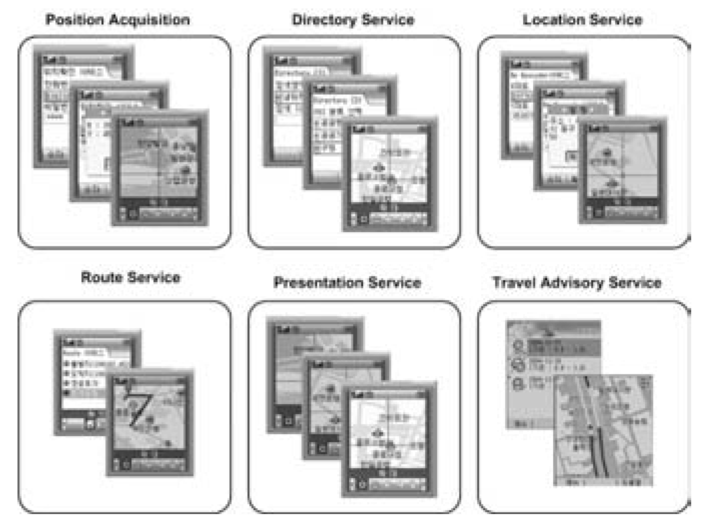
\includegraphics[bb=0 0 706 527, scale=0.45]{figure/fig13.png}
		\captionof{figure}{LBS移动客户端(WIPI:Wireless Internet Platform for Interoperability)}
	\end{minipage}

	\noindent\begin{minipage}{\textwidth}
		\centering
		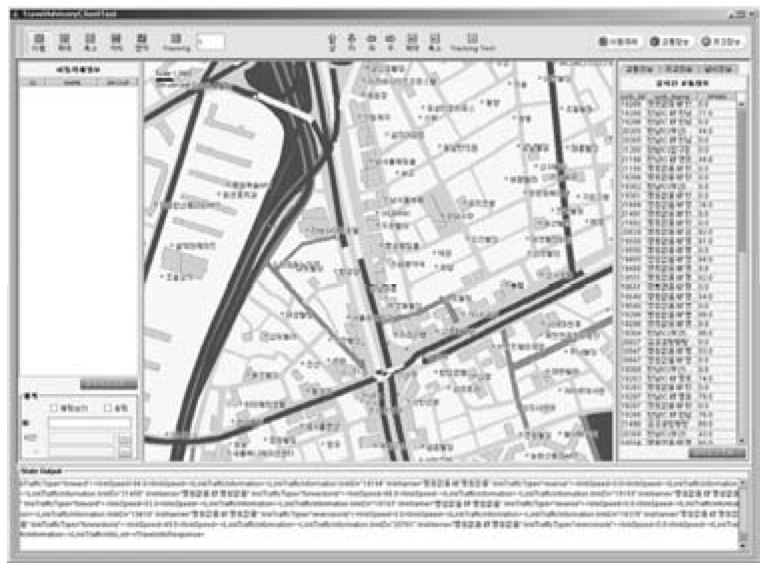
\includegraphics[bb=0 0 768 573, scale=0.45]{figure/fig14.png}
		\captionof{figure}{旅游咨询服务客户端}
	\end{minipage}

	\noindent\begin{minipage}{\textwidth}
		\centering
		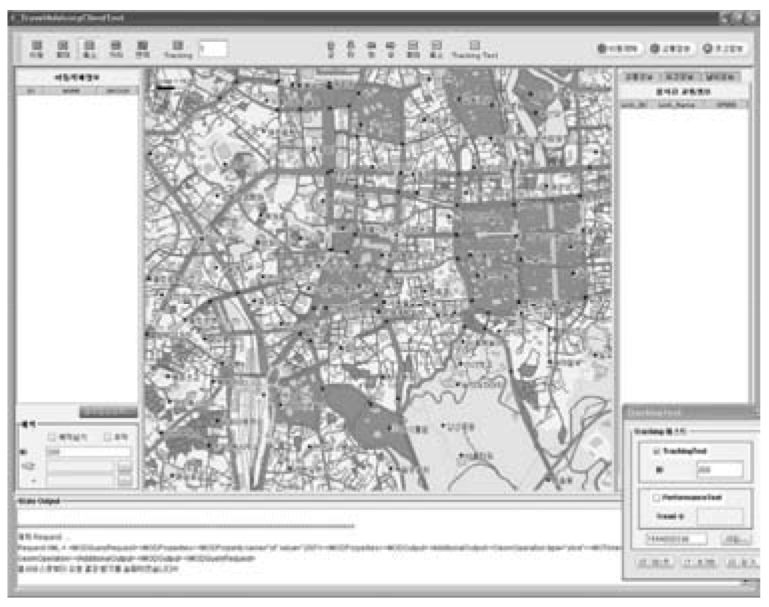
\includegraphics[bb=0 0 769 607, scale=0.45]{figure/fig15.png}
		\captionof{figure}{跟踪服务客户端}
	\end{minipage}

	\noindent\begin{minipage}{\textwidth}
		\centering
		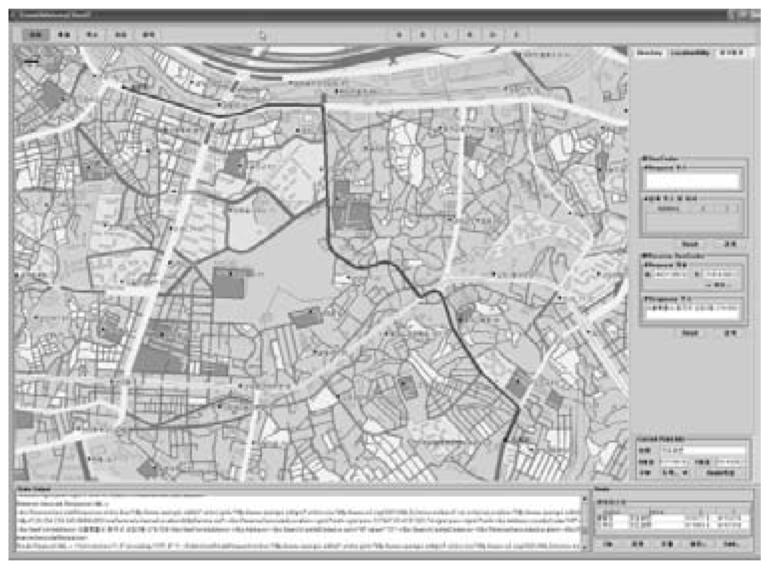
\includegraphics[bb=0 0 770 569, scale=0.45]{figure/fig16.png}
		\captionof{figure}{导航服务客户端(路径导航服务,展示服务,位置实用工具服务,目录服务)}
	\end{minipage}


	\section{结论}
	本论文中提出的LBS基本核心Web服务克服了平台的依赖性,同时提高了分布式计算性能。该基本核心服务不依赖服务器平台,不会因为服务器平台的不同而需重新架构。并且由于采用Web服务系统架构,客户端的开发并不会受限于编程语言。


	% Import references datas
	\bibliography{references.bib}

	\end{CJK}
\end{document}
